%!TEX root = ../thesis.tex

\chapter{深对流对氮氧化物垂直分布的影响}

\section{模式设置}

\subsection{气象及化学设置}

\subsection{闪电参数化}

% \section{模式评估}


\section{结果与讨论}

\subsection{云上二氧化氮柱密度的分布}

由上一章分析可知,将卫星观测所得的NO$_2$柱密度和闪电数据相结合,可以得出LNO$_2$的产率,然而NO$_2$的垂直分布无法由此直接得出。
因此本章将采用云切片的方法,利用卫星针对不同高度深厚对流云的观测,得到云间的平均NO$_2$浓度,从而获得对流状态下的NO$_2$平均廓线,并与全球模式进行对比分析。

图\ref{fig:no2geo_tropomi}为TROPOMI观测的2019年中低纬度云上NO$_2$分布图,
云的中心气压分别为330 hPa、450 hPa、570 hPa、670 hPa、770 hPa、以及 870 hPa。
其中330 hPa和450 hPa的云上NO$_2$高值区位于美国东南部、中国沿海地区、中国华北地区、墨西哥、巴拿马、
古巴、孟加拉国、尼泊尔、新德里、非洲中部、和热带辐合带,
这些地区与图\ref{fig:no2_ltngcount}(c)的闪电高值区相对应。
前人研究表明,中低纬LNO$_2$的峰值分布在100--500 hPa之间\citep{Pickering.1988,Ott.2010,Luo.2017},
故330 hPa和450 hPa的云上NO$_2$包含了LNO$_2$的贡献。
然而TROPOMI的晴空NO$_2$平均柱密度产品显示(图\ref{fig:no2_ltngcount}b),这些地区属于NO$_2$高污染区,所以上对流层的NO$_2$也有来自深对流垂直输送的污染NO$_2$。
中云(570 hPa和670 hPa)的云上NO$_2$有效数据更多,云上NO$_2$高值区包含了高云(330 hPa和450 hPa)的云上NO$_2$高值区。
其中污染NO$_2$的贡献更为明显,与晴空NO$_2$平均柱密度产品分布更为接近,如中国东部、欧洲、和美国东北部的工业源以及非洲中部的生物质燃烧。
污染物排放在低云(770 hPa和870 hPa)的云上NO$_2$最为明显,然而由于热带地区云顶较高,有效数据更少。


\begin{figure}[!htbp]
    \centering
    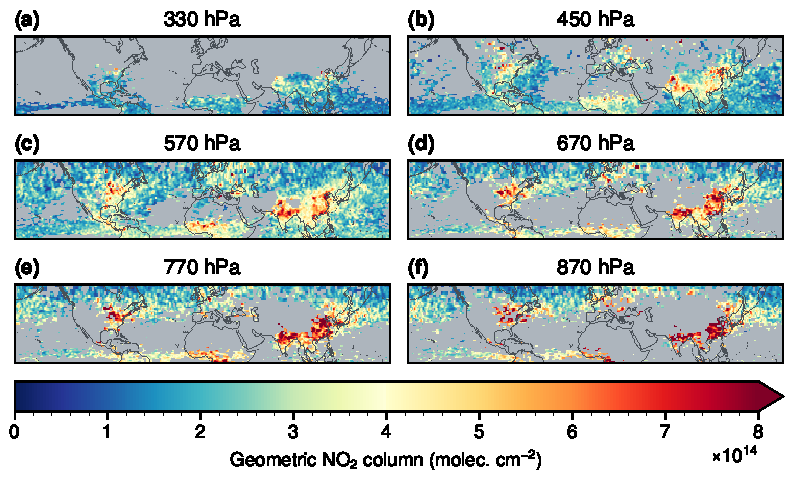
\includegraphics[width=15cm]{./figures/no2geo_tropomi.pdf}
    \caption{
    2019年6--8月北半球中低纬度TROPOMI观测的云上NO$_2$柱密度分布图:
    高云([a] 330 hPa 和 [b] 450 hPa),中云 ([c] 570 hPa 和 [d] 670 hPa),
    及低云 ([e] 770 hPa 和 [f] 870 hPa)。 \\
    NO$_2$ above cloud at the middle and low latitudes for June--August in 2019:
    High clouds ([a] 330 hPa, [b] 450 hPa), middle clouds ([c] 570 hPa, [d] 670 hPa),
    and low clouds ([e] 770 hPa, [f] 870 hPa).
    }
    \label{fig:no2geo_tropomi}
\end{figure}


\begin{figure}[!htbp]
    \centering
    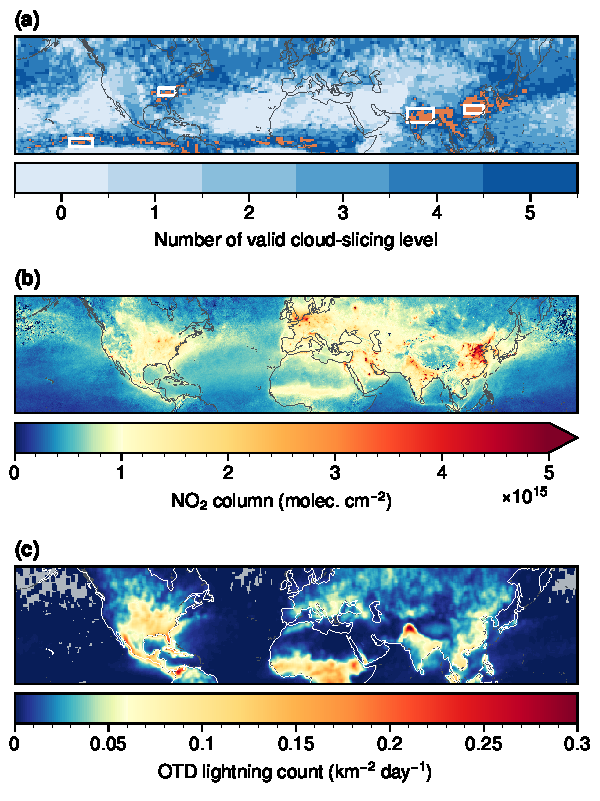
\includegraphics[width=13cm]{./figures/no2_ltngcount.pdf}
    \caption{
    (a) 云切片的总有效气压层数,层数$\leq$ 5为蓝色,= 6 为橙色,白色方框为NO$_2$廓线选区(图\ref{fig:utno2_profile})。
    (b)2019--2021年中低纬度夏季(6--8月)TROPOMI测得的NO$_2$平均柱密度。
    (c) 1995--2014年中低纬度夏季(6--8月)LIS/OTD的闪电密度产品。 \\
    (a) Number of total valid cloud-slicing pressure levels.
    Grids with number of levels $leq$ 5 and = 6 are filled in blue and orange, respectively.
    White rectangles are selections for NO$_2$ profiles (Fig. \ref{fig:utno2_profile}).
    (b) The average TROPOMI NO$_2$ column densities at the middle and low latitudes for June--August in 2019--2021.
    (c) The average LIS/OTD lightning flash rates at the middle and low latitudes for June--August in 1995--2014.
    }
    \label{fig:no2_ltngcount}
\end{figure}

\subsection{二氧化氮的垂直分布}


上节得到的云上NO$_2$为对流层NO$_2$柱密度,柱底为云的中心气压,
通过\ref{sec:云切片算法}章的云切片算法可进一步得到每层的NO$_2$浓度,即NO$_2$廓线。

图\ref{fig:utno2_tropomi}为2019年6--8月不同高度的NO$_2$平均浓度。
与图\ref{fig:no2geo_tropomi}不同,高云处的NO$_2$浓度(图\ref{fig:utno2_tropomi}(a--b))高于中云(图\ref{fig:utno2_tropomi}(c--d))。
其中陆地上180 hPa--330 hPa间的NO$_2$为330 hPa--450 hPa间的$\approx$1.2倍,为450--570 hPa间的$\approx$2倍,
而570 hPa以下(图\ref{fig:utno2_tropomi}(d--f))陆地上的NO$_2$浓度逐渐上升。
该现象与前人的模拟和飞机观测结果相符,LNO$_2$在上对流层占主导,而污染NO$_2$在下对流层占主导\citep{Pickering.1996,Ott.2010,Laughner.2017}。


\begin{figure}[!htbp]
    \centering
    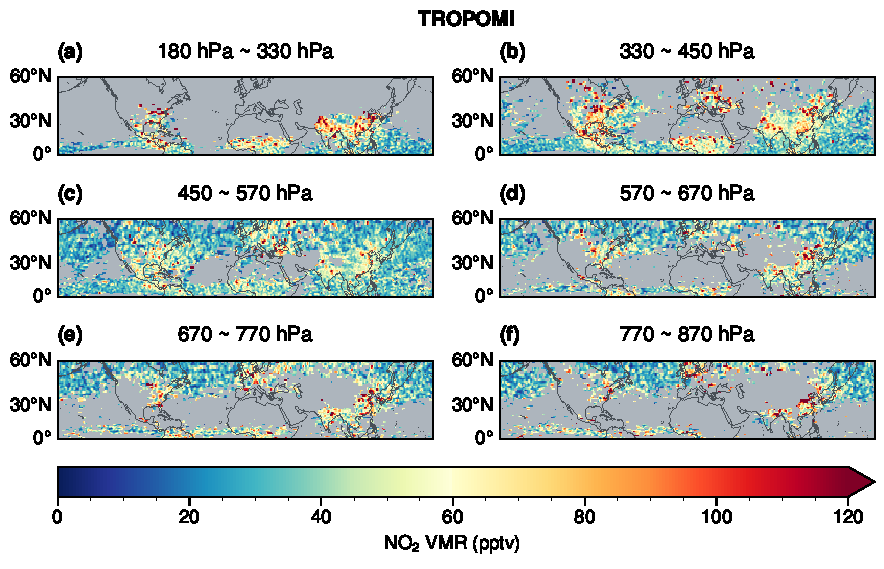
\includegraphics[width=15cm]{./figures/utno2_tropomi.pdf}
    \caption{
    TROPOMI云切片算法所得的2019年6--8月北半球中低纬度NO$_2$浓度分布图。 \\
    The NO$_2$ vertical mixing ratios derived from the cloud-slicing results of TROPOMI NO$_2$ observations at the northern middle and low latitudes for June--August in 2019.
    }
    \label{fig:utno2_tropomi}
\end{figure}


为了进一步分析LNO$_2$在其中的作用,我们首先将各个高度层的TROPOMI观测结果与MERRA2-GMI的模式结果相比较,
接着选取TROPOMI云切片各层均有有效数据的区域,结合过境期间模拟的LNO$_2$排放速率垂直分布进行廓线分析。
图\ref{fig:utno2_merra2}为2019年6--8月与TROPOMI对应的MERRA2-GMI NO$_2$模拟结果。
由两者浓度之差(图\ref{fig:utno2_delta})可知,无论位于陆地还是海洋,MERRA2-GMI较TROPOMI存在20--80 pptv的低估,
其中海洋上的误差可能由TROPOMI NO$_2$反演过程中低估的平流层NO$_2$柱密度或高估的辐射强度所导致\citep{VanGeffen.2020}。


\begin{figure}[!htbp]
    \centering
    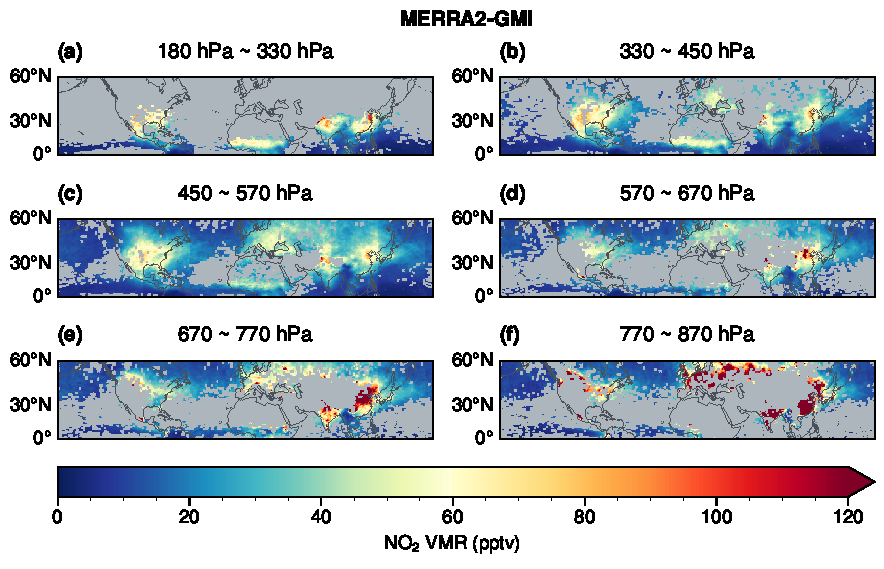
\includegraphics[width=15cm]{./figures/utno2_merra2-gmi.pdf}
    \caption{
    同图\ref{fig:utno2_tropomi}但数据为MERRA2-GMI。 \\
    Same as Fig. \ref{fig:utno2_tropomi} but for MERRA2-GMI.
    }
    \label{fig:utno2_merra2}
\end{figure}

\begin{figure}[!htbp]
    \centering
    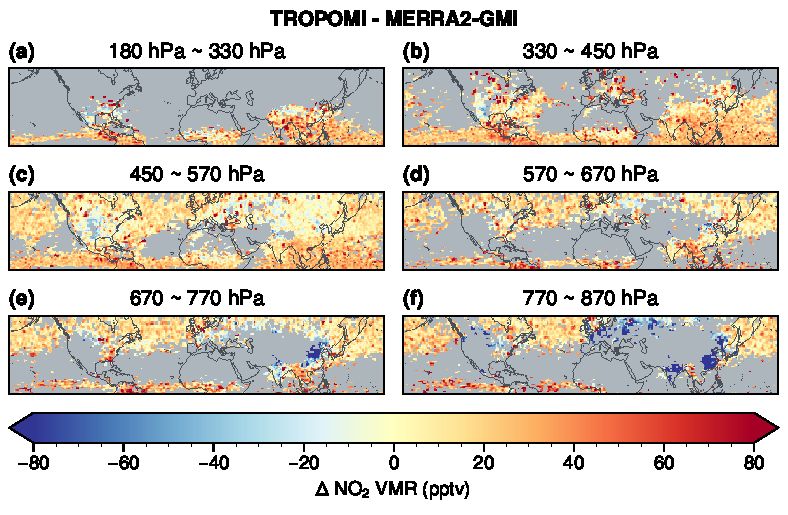
\includegraphics[width=15cm]{./figures/utno2_delta.pdf}
    \caption{
    图\ref{fig:utno2_tropomi}与图\ref{fig:utno2_merra2}之差。 \\
    Differences between Fig. \ref{fig:utno2_tropomi} and Fig. \ref{fig:utno2_merra2}.
    }
    \label{fig:utno2_delta}
\end{figure}


具体而言,高云间的NO$_2$正误差结果($\Delta$ NO$_2$ $>$ 0,图\ref{fig:utno2_delta}a和b)主要来自于北美、东欧、以及亚洲东部沿海,
这意味着MERRA2-GMI全球模式中参数化对流垂直传输污染物的强度较低,导致高云间的NO$_2$低于TROPOMI的观测值。
而高云间的NO$_2$负误差结果位于美国中部,非洲中部,以及青藏高原西南部。
美国中部和非洲中部的误差是由于MERRA2-GMI中的闪电参数化(上对流层的向上云质量通量)在该区域高估了闪电总量,从而导致NO$_2$浓度偏大\citep{Allen.2002,Allen.2010}。
由LIS/OTD数据(图\ref{fig:no2_ltngcount}c)可知,青藏高原西南部闪电强度较弱,故模式的高估主要应来自于亚洲夏季风的污染物输送。

中云的云切片结果有效范围最广,总体上来看TROPOMI和MERRA2-GMI之间误差较低(-10--30 pptv),
且两者具有相似的高值区分布:北美、东欧、印度、以及中国华北地区,这些地区与污染NO$_2$柱密度高值区对应。
中云的NO$_2$可能来源有对流输送的地表污染和污染的出流区,如中国华北地区的NO$_2$高值传输至东部的黄海(其中一部分也来自于船舶排放)。
其中$>$ 40 pptv的正误差集中于南美洲北部、缅甸、和泰国北部,由于这些地区地基NO$_2$稀缺,
所以该误差应归因于卫星反演误差还是模式NO$_x$排放源需更新,有待进一步研究。
此外,中云的负误差结果在570--670 hPa更为明显,尤其是中国的华北地区,考虑到MERRA2-GMI对流垂直输送强度较低,故而使用的排放清单中NO$_x$排放量可能过高\citep{Ziemke.2019}。

低云的云切片结果NO$_2$高值区与中云结果类似,值得注意的是云切片结果比MERRA2-GMI的数据低50--200 pptv,
该差异在中国东部和印度北部最为明显($>$ 100 pptv)。
前人研究表明,几何AMF(AMF$_{geo}$)在低云和污染条件下可达可见AMF(AMF$_{Vis}$,公式\ref{eq:AMF_NO2Vis})的两倍\citep{BelmonteRivas.2015},然而不足以解释中国东部地区的模拟值为观测值的3--5倍。
因此,该差异反映了MERRA2-GMI使用的大气化学和气候模型比对项目 (ACCMIP) 排放清单在中国东部未能及时更新。

除了各层NO$_2$浓度的地理分布之外,我们选取了区域内云切片有效层数为6层的格点(中国南部、印度中部、美国东南部、以及太平洋,图\ref{fig:no2_ltngcount}a),
进行TM5、MERRA2-GMI,和TROPOMI的廓线对比分析,
其中TM5的NO$_2$廓线为TROPOMI官方产品使用的TM5全球模式先验廓线(包含TROPOMI同化)。
由于TROPOMI在太平洋清洁地区的高估,我们将云切片结果进行校正,即除以其与MERRA2-GMI和TROPOMI比例的平均值。
如图\ref{fig:utno2_profile}所示,太平洋清洁地区NO$_2$在对流层各层浓度均一(2.5--12.5 pptv),中国南部和印度中部低层NO$_2$污染浓度高(200--300 pptv),而美国东南部低层NO$_2$浓度处于50--100 pptv。
在污染地区低层,TROPOMI存在与图\ref{fig:utno2_delta}中类似的低估,故只比较三者在对流层中上层的NO$_2$浓度。
对于中国南部、印度中部、和美国东南部,NO$_2$浓度均随高度而下降,在500--600 hPa存在转折点,进而浓度上升,在180--300 hPa达到峰值。
总体来看,对流层中上层MERRA2-GMI和TM5的NO$_2$浓度相近,但均低于TROPOMI的结果,
表明模式中LNO$_2$或闪电参数化存在低估,与前人的飞机探测和模式结果相符\citep{Laughner.2019a,Zhang.2022a}。
此外,TM5的中上层拐点梯度更高,最上层的NO$_2$浓度较MERRA2-GMI更接近TROPMI的结果,这是由于TM5的同化缺失了云下的信息。
虽然MERRA2-GMI在美国东南部的LNO$_2$排放速率为中国南部或印度中部的两倍,但是最上层的峰值浓度与TM5一致($\approx$60 pptv),不同之处为浓度拐点降为700 hPa,该高度低于TM5和TROPOMI的500 hPa,可能原因是MERRA2-GMI的LNO$_2$排放廓线在美国东南部的中低层权重过高。
总之,TROPOMI的观测结果和MERRA2-GMI/TM5的模拟结果在对流层中上层存在显著的一致性,
局部的差异表明云切片方法可以用来检验模式的对流垂直输送和水平输送能力,LNO$_x$的产量和分布、以及使用的排放源清单。


\begin{figure}[!htbp]
    \centering
    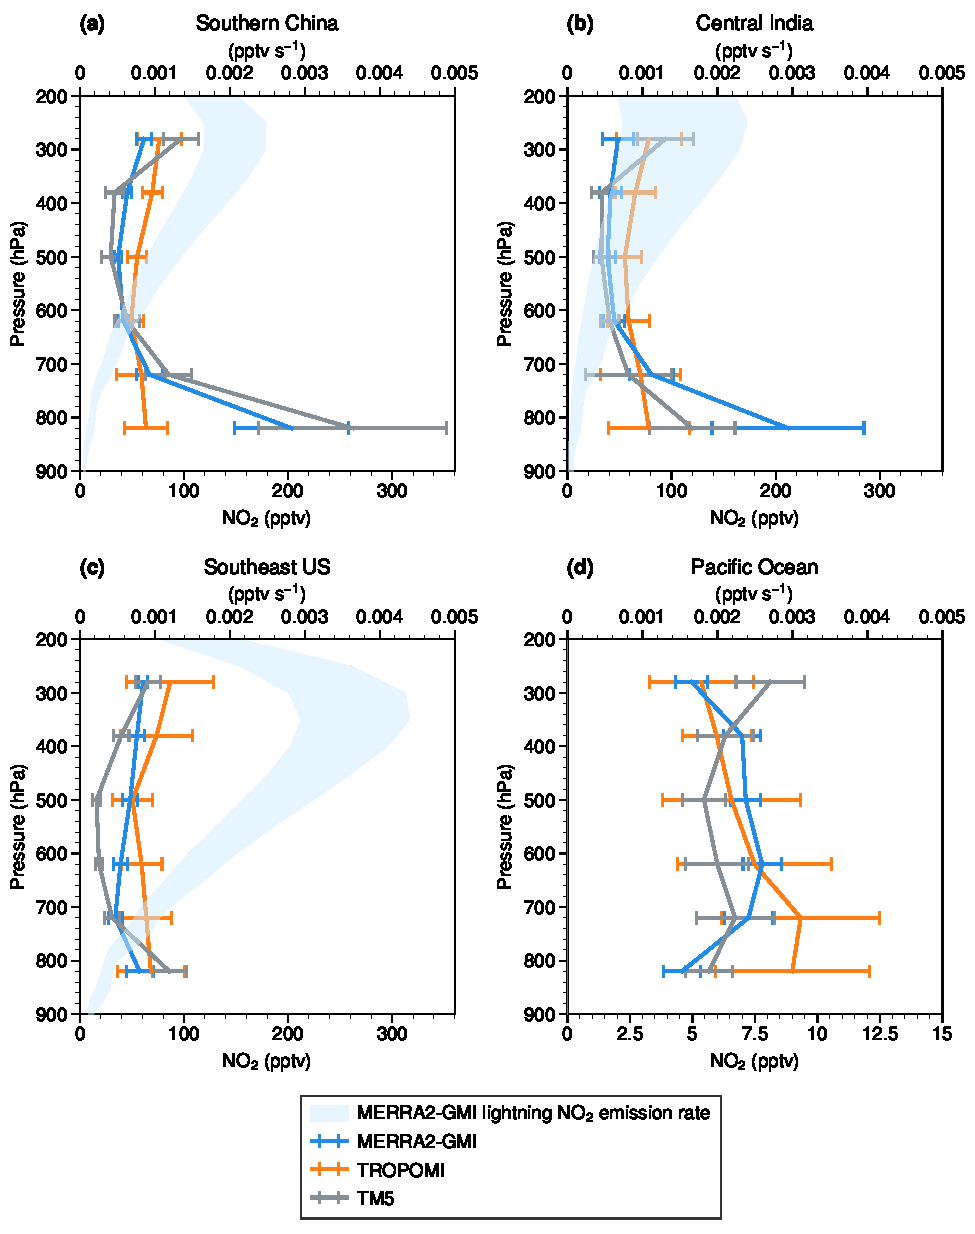
\includegraphics[width=12cm]{./figures/utno2_profile.pdf}
    \caption{
    TM5(灰色)、MERRA2-GMI(蓝色)、以及TROPOMI云切片算法(橙色)所得到的区域平均NO$_2$廓线
    (a)中国南部、(b)印度中部、(c)美国东南部、(d)太平洋(区域示意图见图\ref{fig:no2_ltngcount}a)。
    浅蓝色填充部分为下午地方时2点的MERRA2-GMI闪电NO$_2$排放速率,
    其中廓线的误差棒和填充范围为平均值$\pm$标准差。\\
    Regional average NO$_2$ profiles obtained by TM5 (gray), MERRA2-GMI (blue), and TROPOMI cloud slice algorithm (orange)
    (a) southern China, (b) central India, (c) southeastern United States, and (d) Pacific Ocean
    (Definitions of region are shown in Fig. \ref{fig:no2_ltngcount}a).
    The light blue filled part is the MERRA2-GMI lightning NO$_2$ emission rate at local 2 p.m.,
    where the error bars and filled ranges of the profiles are the mean values $\pm$ standard deviations.
    }
    \label{fig:utno2_profile}
\end{figure}



% \subsection{闪电氮氧化物的影响} \label{subsect:lnox_affects_tropomi}
% \subsection{不同排放源对氮氧化物垂直分布的贡献}
\subsection{闪电氮氧化物对TROPOMI产品的影响}  \label{subsect:lnox_affects_tropomi}

鉴于LNO$_2$在对流层中上层的主导地位和更长寿命,我们接着探讨了LNO$_x$对官方NO$_2$柱浓度产品的影响。
图\ref{fig:flash_scd}(a--d)将对流层NO$_2$斜柱浓度(S$_{\textrm{NO$_2$}}$)的分布与观测的闪电分布进行了比较。
尽管由于探测器饱和和光晕效应,闪电最活跃像素上的S$_{\textrm{NO$_2$}}$无效,但附近或对流出流区仍有有效数据。
在2019年的个例中,闪电发生在TROPOMI过境前不到30分钟,但2020年的个例中既有新生的也有老化的LNO$_2$(图\ref{fig:flash_scd}(d))。

\begin{figure}[!htbp]
    \centering
    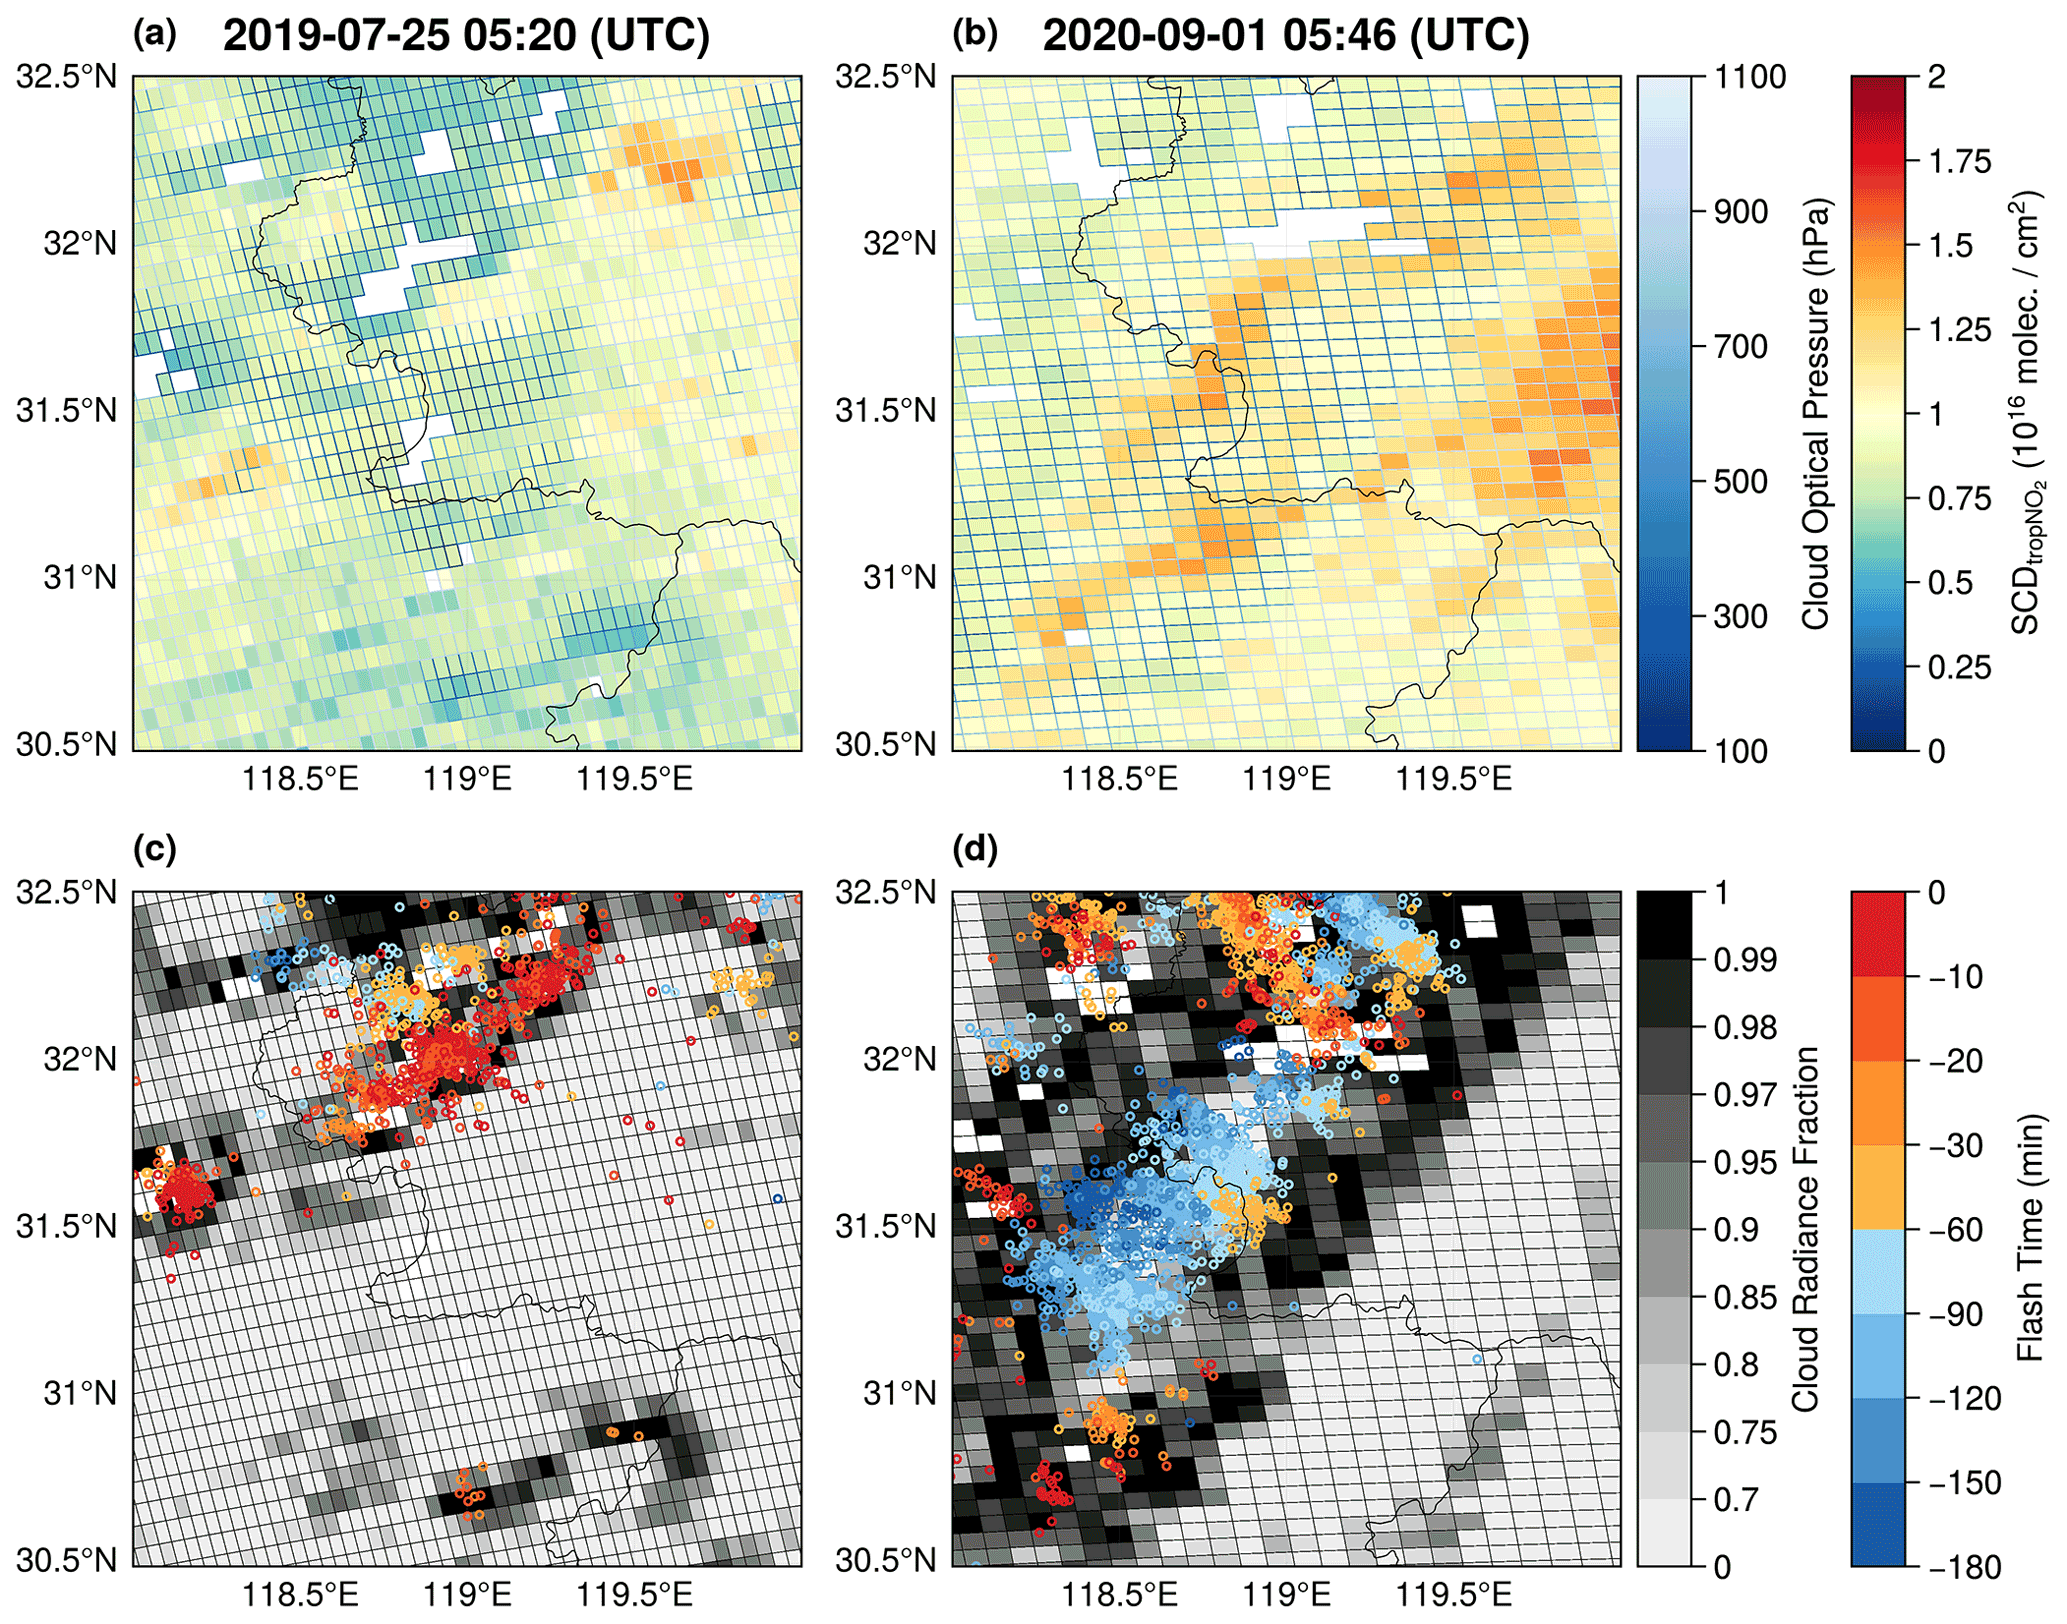
\includegraphics[width=12cm]{./figures/flash_scd.png}
    \caption{
    2019 年 7 月 25 日(左)和 2020 年 9 月 7 日(右)的个例。
    (a, b) 对流层 NO$_2$ 斜柱密度(SCD$_\textrm{tropNO$_2$}$,填充色)和云压(线条颜色)。
    这些白色网格单元代表缺失的 TROPOMI 数据,黑色实线为江苏省。
     (c, d) NO$_2$ 窗区中的云辐射分数和闪电。闪电的颜色取决于相对于TROPOMI过境的发生时间。\\
    Figure \ref{fig:flash_scd}. Events on 25 July 2019 (left) and 07 September 2020 (right).
    (a, b) The tropospheric NO$_2$ slant column density (SCD$_\textrm{tropNO$_2$}$, filled color) and cloud optical pressure (line color).
    These white grid cells stand for missing TROPOMI data.
    The solid black border is Jiangsu province.
    (c, d) The cloud radiance fraction in the NO$_2$ window and flashes whose color depends on the occurring time relative to the TROPOMI overpass time.
    }
    \label{fig:flash_scd}
\end{figure}

具体而言,对流旺盛处(f$_r$ $\geq$ 0.7)的S$_{\textrm{NO$_2$}}$小于其他区域。
这与之前针对具有高闪电密度的大规模对流系统的研究结果相反\citep{Beirle.2009}。
导致这一差距的因素有四点:云顶高度、闪电次数、闪电发生时间和背景NO$_2$浓度。
由于TROPOMI只能探测到处于云层上方的LNO$_2$,因此当fr $\approx$ 1时,闪电次数不足或对流较弱都可能导致对流旺盛区的S$_{\textrm{NO$_2$}}$更小。
即如果f$_r$<1,则破碎或稀薄云层下方的污染NO$_2$则会部分被TROPOMI探测到。
而WRF-Chem的先验S$_{\textrm{NO$_2$}}$敏感性试验可以清楚地解释这种现象(图\ref{fig:s5p_apriori_scd})。
具有低f$_r$和高S$_{\textrm{NO$_2$}}$像素源自于背景 NO$_2$ 污染(图\ref{fig:s5p_apriori_scd}(a)和(e)),
但与没有LNO$_2$贡献的低S$_{\textrm{NO$_2$}}$相比,上对流层LNO$_2$增加的S$_{\textrm{NO$_2$}}$仍然可见(图\ref{fig:s5p_apriori_scd}(b)--(d) 和 (f)--(h))。

\begin{figure}[!htbp]
    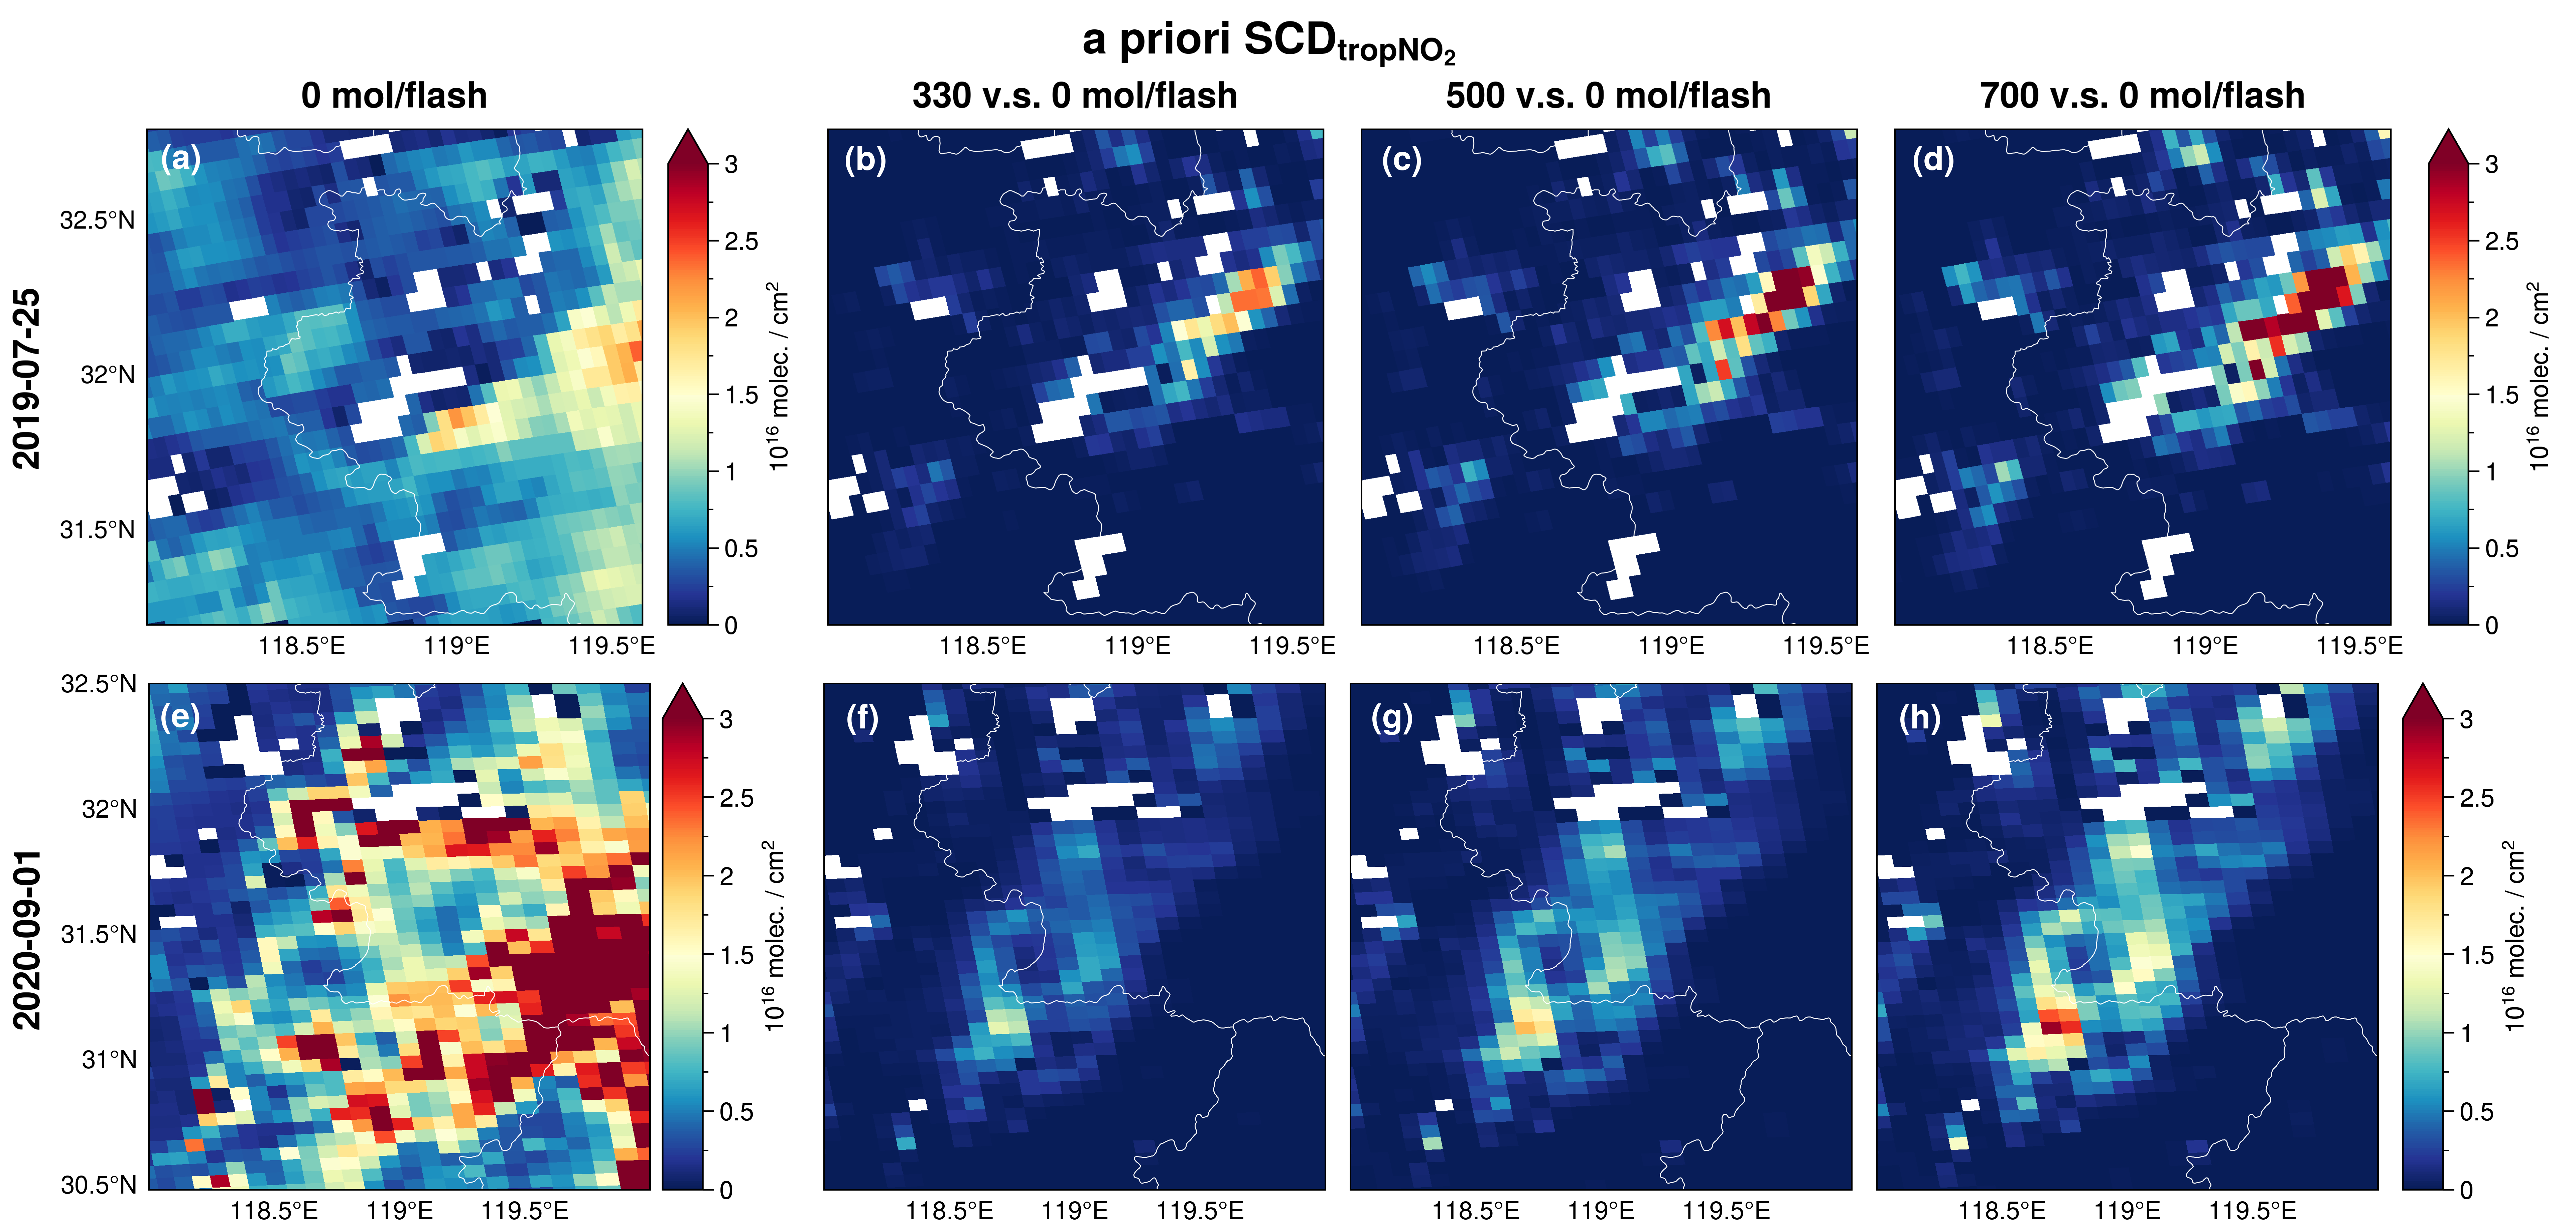
\includegraphics[width=17cm]{./figures/s5p_apriori_scd.png}
    \caption{使用不同闪电NO排放的WRF-Chem结果,重新计算得到的对流层NO$_2$斜柱密度 (SCD$_\textrm{tropNO$_2$}$):
    Figure \ref{fig:s5p_apriori_scd}. (a, e) 0 mol每闪电, (b, f ) 330 mol每闪电, (c, g) 500 mol每闪电 和 (d, h) 700 mol每闪电。\\
    The tropospheric NO$_2$ slant column density (SCD$_\textrm{tropNO$_2$}$) recalculated using the WRF-Chem results with different lightning NO settings: (a, e) 0 mol/flash, (b, f) 330 mol/flash, (c, g) 500 mol/flash and (d, h) 700 mol/flash.
    }
    \label{fig:s5p_apriori_scd}
\end{figure}


为了研究LNO$_x$对AMF$_\textrm{trop}$和AMF$_\textrm{LNO$_x$}$计算的重要性,我们将LNO产率的上限700 mol NO 每闪电\citep{Ott.2010}应用于WRF-Chem 。
接着我们通过独立替换三个对流层层中的NO$_2$廓线:对流层中层(MT,800 到 400 hPa)、对流层上层(UT,400 到 150 hPa)和整个对流层(地表到对流层顶)。
除非另有说明,否则后文AMF的变化是通过增加LNO$_x$获得的。
如图\ref{fig:s5p_amf_diff}显示,AMF变化主要由检测灵敏度高的上对流层LNO$_x$所控制\citep{Beirle.2009,Laughner.2017},且LNO$_x$产量在该高度达到峰值(图\ref{fig:nox_profile})。
虽然两种情况下AMF均降低了5\%--40\%,但AMF$_\textrm{trop}$的变化($\Delta$AMF$_\textrm{LNO$_x$}$)具有区域特异性。
可根据闪电活动对其进行分类:新生闪电区(MT ΔAMF\%)、闪电下风向(MT $\Delta$AMF$_\textrm{trop}$>20\%)和闪电老化区(UT $\Delta$AMF$_\textrm{trop}$>20\%)。
图\ref{fig:amf_contribution}(a)说明了云压(p$_{cloud}$)和f$_r$在这三个区域上的关系。
云层高于400 hPa(p$_{cloud}$< 400 hPa),新生闪电区的像素上f$_r$大于0.8,但闪电老化区和闪电下风向都有低于400 hPa的云层。
这与图\ref{fig:nox_profile}中的平均云压一致,并解释了为什么UT $\Delta$AMF$_\textrm{trop}$ > 20\% 在图\ref{fig:s5p_amf_diff}(b)i 和 (b)iii 中存在,这也正表明了在闪电老化区估算LNO$_x$的可能性。


\begin{figure}[!htbp]
    \centering
    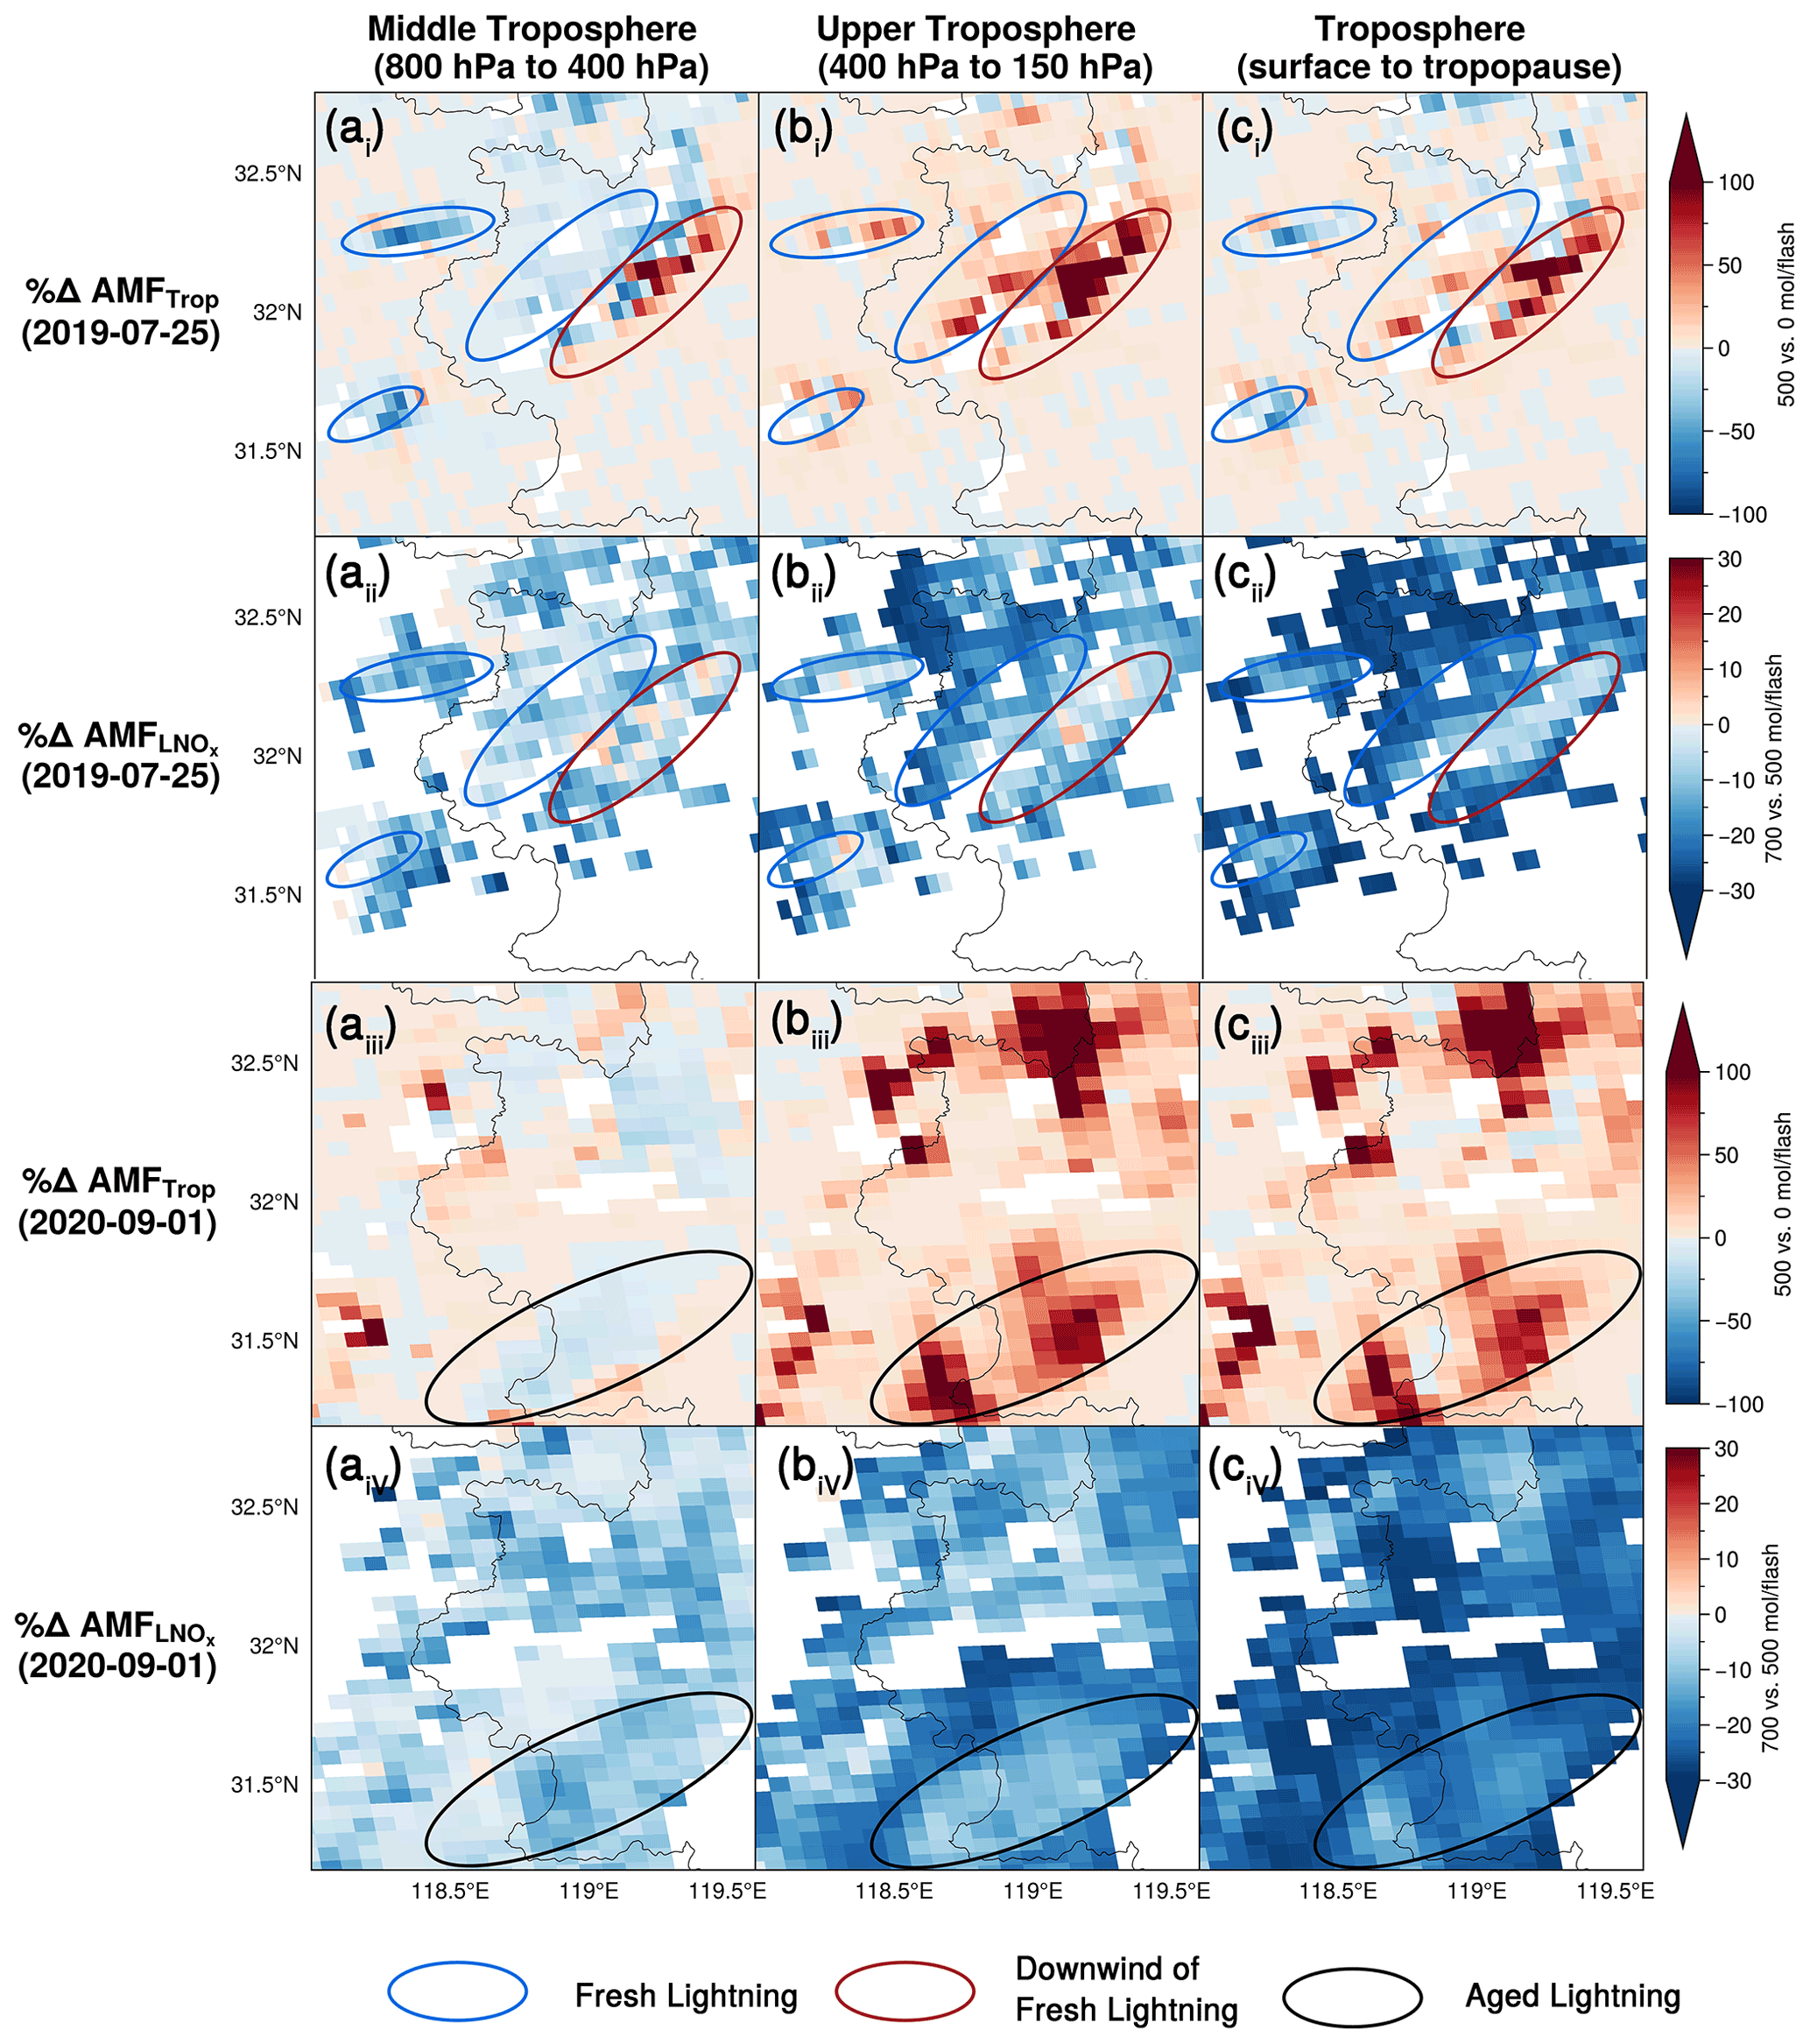
\includegraphics[width=12cm]{./figures/s5p_amf_diff.png}
    \caption{
    通过替换三层的NO$_2$先验廓线,得到的空气质量因子(AMF)百分比差异:三层具体为:对流层中层(左)、对流层上层(中)和整个对流层(右)。
     $\Delta$AMF$_\textrm{trop}$ 是 500 mol NO/闪电得到的AMF$_\textrm{trop}$ 与0 mol NO/闪电得到的AMF$_\textrm{trop}$之差。
     $\Delta$AMF$_\textrm{LNO$_x$}$ 是 500 mol NO/闪电得到的AMF$_\textrm{LNO$_x$}$ 与0 mol NO/闪电得到的AMF$_\textrm{LNO$_x$}$之差。
     标注了三个区域:新生闪电区(蓝色),闪电下风向(红色),和闪电老化区(黑色)。\\
    Figure \ref{fig:s5p_amf_diff}. The percent differences of AMFs by replacing the a priori NO$_2$ profiles at three layers:
    middle troposphere (left), upper troposphere (middle), and troposphere (right).
    $\Delta$AMF$_\textrm{trop}$ is the comparison of the AMF$_\textrm{trop}$ with 500 mol NO per flash relative to 0 mol NO per flash.
    $\Delta$AMF$_\textrm{LNO$_x$}$ is the comparison of the AMF$_\textrm{LNO$_x$}$ with 700 mol NO per flash relative to 500 mol NO per flash.
    Three regions are annotated: fresh lightning (blue),
    downwind of fresh lightning (red),
    and aged lightning (black).
    % Because of the quite large AMF$_\textrm{LNO$_x$}$ values in pixels with little lightning,
    % $\Delta$AMF$_\textrm{LNO$_x$}$ is shown over pixels where 0 $<$ AMF$_\textrm{LNO$_x$}$ $<$ 10.
    }
    \label{fig:s5p_amf_diff}
\end{figure}


\begin{figure}[!htbp]
    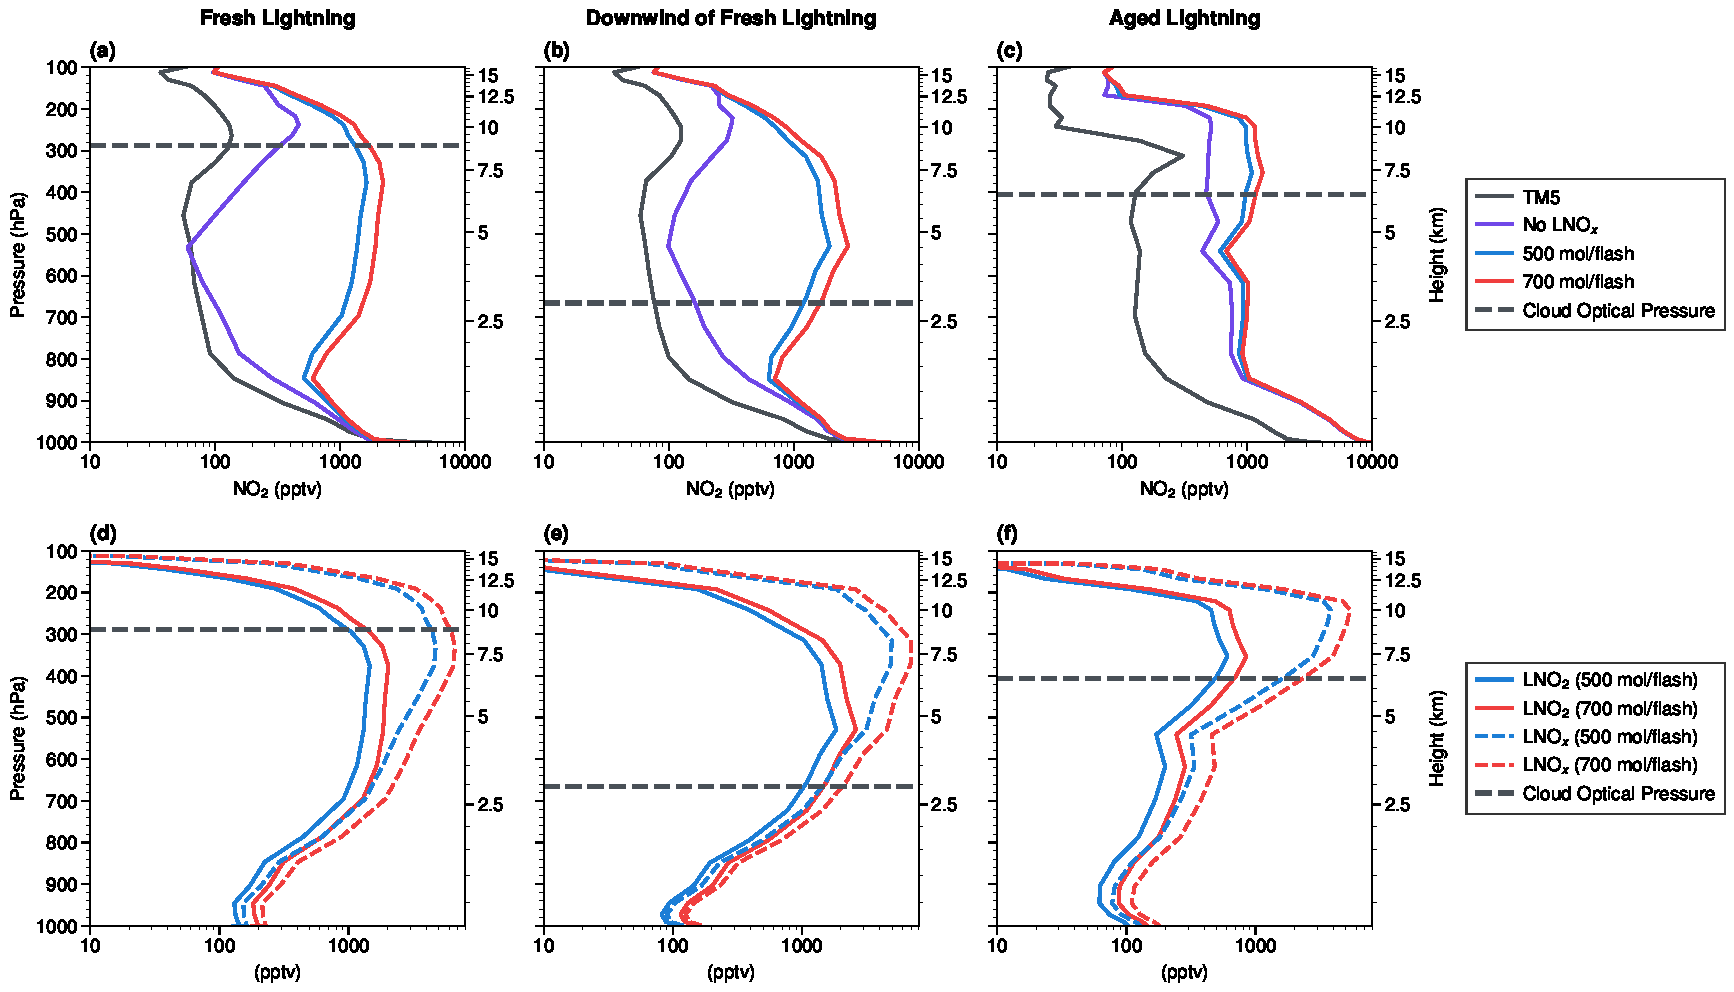
\includegraphics[width=17cm]{./figures/nox_profile.pdf}
    \caption{
    TROPOMI过境时,在不同闪电NO的排放条件下,三个区域(新生闪电区,闪电下风向,和闪电老化区)的各物质垂直廓线。
     (a--c) NO$_2$廓线与官方TM5先验NO$_2$廓线之间的比较。
     (d--f) 闪电 NO$_2$ 和 NO$_x$廓线。灰色虚线是TROPOMI探测到的云压。\\
     Figure \ref{fig:nox_profile}. Profiles with different lightning NO productions at TROPOMI overpass time over three regions (fresh lightning, downwind of fresh lightning, and aged lightning).
    (a--c) The NO$_2$ profiles compared with the official TM5 a priori NO$_2$ profile.
    (d--f) The lightning NO$_2$ and NO$_x$ profiles.
    The gray dashed line is the cloud optical pressure detected by TROPOMI.
    }
    \label{fig:nox_profile}
\end{figure}


\begin{figure}[!htbp]
    \centering
    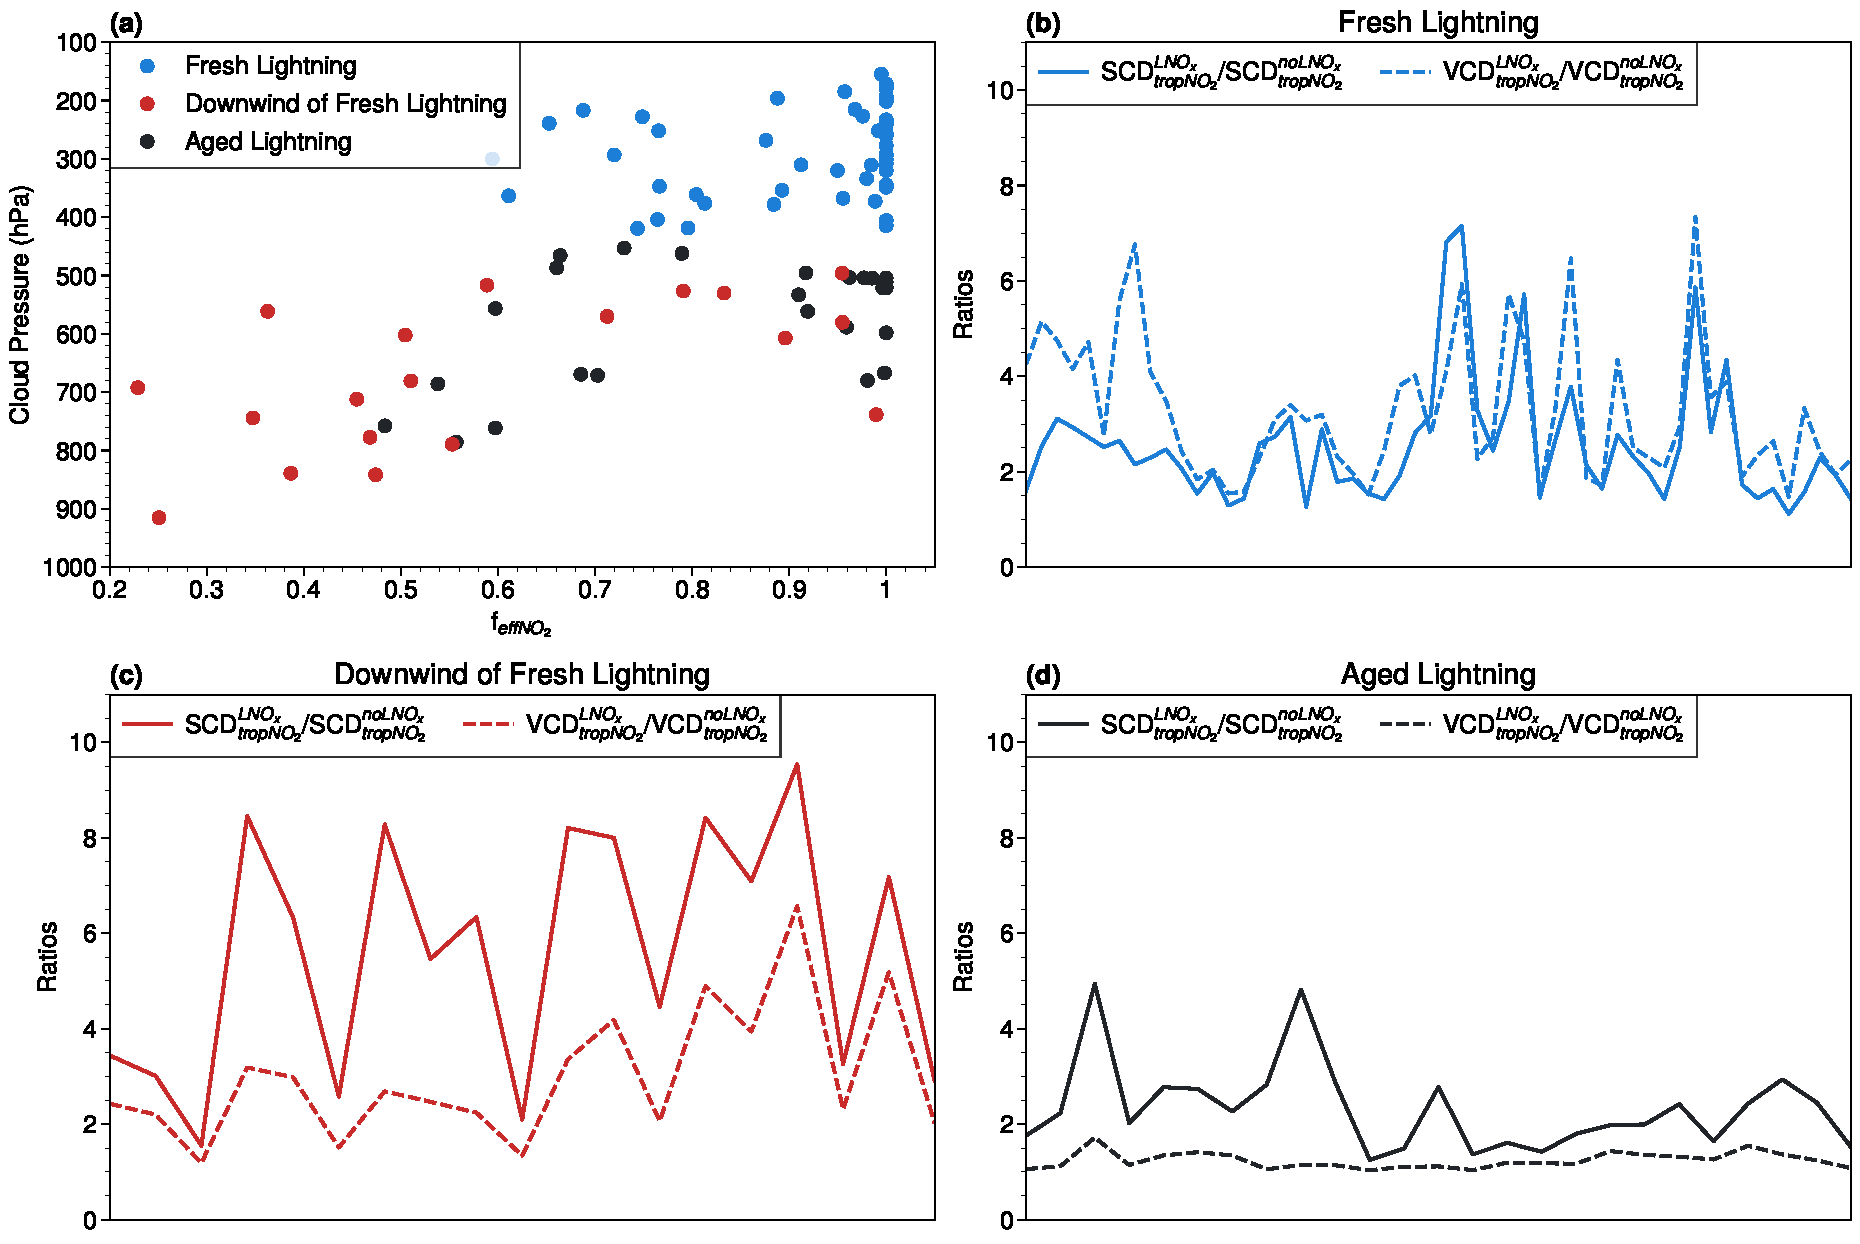
\includegraphics[width=14cm]{./figures/amf_contribution.pdf}
    \caption{
    (a) 图 \ref{fig:s5p_amf_diff} 中定义的三个区域(新生闪电区,闪电下风向,和闪电老化区)的云压和云辐射分数之间的关系。
     (b--d) 这三个区域的先验SCD$^{\textrm{LNO$_x$}}_{\textrm{tropNO$_2$}}$/SCD$^{\textrm{noLNO$_x$}}_{ \textrm{tropNO$_2$}}$和先验VCD$^{\textrm{LNO$_x$}}_{\textrm{tropNO$_2$}}$/VCD$^{\textrm{noLNO$_x$ }}_{\textrm{tropNO$_2$}}$。
     LNO$_x$的上标表示先验变量是通过开启LNO$_x$排放(每次闪光 500 mol NO)计算得到的,而上标为noLNO$_x$则代表未开启LNO$_x$排放。\\
     Figure \ref{fig:amf_contribution}. (a) The relationship between cloud pressure and cloud radiance fraction for three regions defined in Fig. \ref{fig:s5p_amf_diff}: fresh lightning region, downwind of fresh lightning, and aged lightning area.
    (b--d) The a priori SCD$^{\textrm{LNO$_x$}}_{\textrm{tropNO$_2$}}$/SCD$^{\textrm{noLNO$_x$}}_{\textrm{tropNO$_2$}}$ and a priori VCD$^{\textrm{LNO$_x$}}_{\textrm{tropNO$_2$}}$/VCD$^{\textrm{noLNO$_x$}}_{\textrm{tropNO$_2$}}$ of pixels in these three regions. The LNO$_x$ superscript indicates that the a priori variable is calculated with LNO$_x$ (500 mol NO per flash) and the noLNO$_x$ superscript is without LNO$_x$.
    }
    \label{fig:amf_contribution}
\end{figure}


\section{本章小结}
